
\documentclass[border=10pt]{standalone}
\usepackage{pgfplots}
\begin{document}
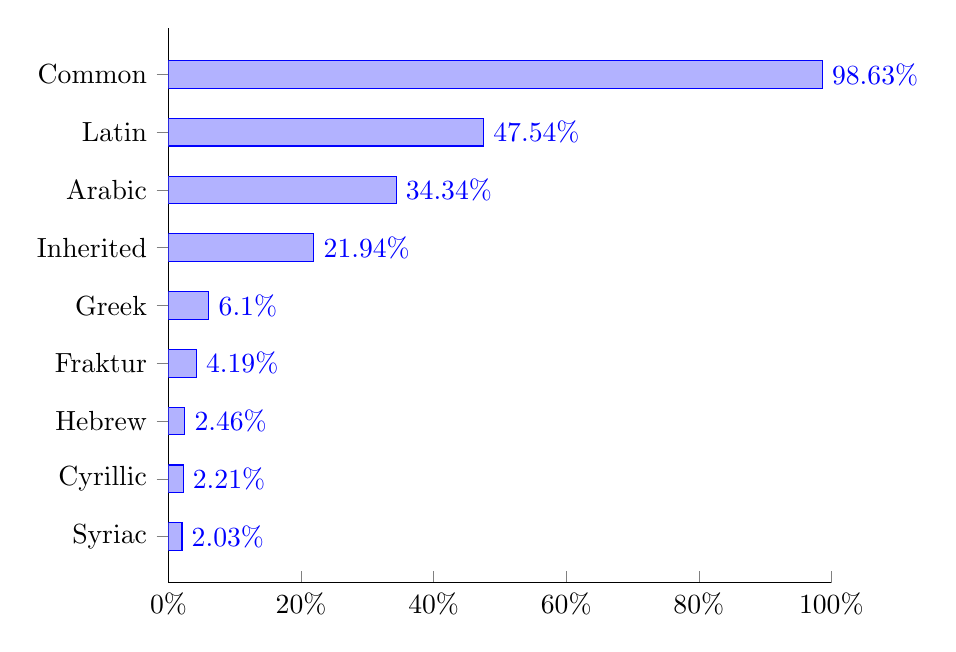
\begin{tikzpicture}
  \begin{axis}[
    axis lines*=left,
    xbar,
    width=10cm,
    xlabel={},
    ytick=data,
    xmin=0,
    xmax=1.0, 
    point meta={x*100},
    nodes near coords={\pgfmathprintnumber\pgfplotspointmeta\%},
    nodes near coords align={horizontal},
    symbolic y coords={Syriac, Cyrillic, Hebrew, Fraktur, Greek, Inherited, Arabic, Latin, Common},
    xticklabel={\pgfmathparse{\tick*100}\pgfmathprintnumber{\pgfmathresult}\%}
  ]

        \addplot coordinates {
		(0.4754016646187374,Latin)
		(0.34335659471866087,Arabic)
		(0.9863213780631999,Common)
		(0.06099738019613753,Greek)
		(0.04194004590452786,Fraktur)
		(0.02455196717130735,Hebrew)
		(0.022071267938701226,Cyrillic)
		(0.020309275960401548,Syriac)
		(0.21936800129830988,Inherited)
        };
  \end{axis}
\end{tikzpicture}
\end{document}
